\documentclass[12pt]{article}
\usepackage[paper=letterpaper,margin=1.5cm]{geometry}
\usepackage{amsmath,amssymb,amsfonts}
\usepackage{newtxtext, newtxmath}
\usepackage{graphicx}
\usepackage{physics}
\usepackage{enumitem}
\usepackage{titling}
\usepackage[colorlinks=true]{hyperref}
\usepackage{autobreak}
\usepackage{listings}
\usepackage[font=small,labelfont=bf]{caption} % Required for specifying captions to tables and figures

\usepackage{graphicx} % Required for the inclusion of images
\graphicspath{{./images/}} % Specifies the directory where pictures are stored

\setlength{\droptitle}{-6em}
\begin{document}

\center
Aprendizagem 2024\\
Homework IV -- Group 016\\
(ist1106022, ist1106720)\vskip 1cm

\large{\textbf{Part I}: Pen and paper}\normalsize
\begin{enumerate}[leftmargin=0pt, label=\textbf{\arabic*.)}]
    \item
          \subsection*{E-step}
          \begin{enumerate}
              \item[a)]
                    $P(x_i \mid c_k) = N(x_i \mid \mu_k, \Sigma_k) = \frac{1}{(2\pi)^{d/2} |\Sigma_k|^{1/2}} e^{-\frac{1}{2} (x_i - u_k)^T \Sigma_k^{-1} (x_i - u_k)}$

              \item[b)]
                    $P(c_k, x_i) = \pi_k \cdot N(x_i \mid \mu_k, \Sigma_k))$

              \item[c)]
                    $P(x_i) = \sum_k (P(c_k, x_i))$ \\
                    $\gamma(c_{ki}) = P(c_k \mid x_i) = \frac{P(c_k , x_i)}{P(x_i)}$

              \item[a)-c)]
                    $\gamma(c_{ki}) = P(c_k \mid x_i) = \frac{P(x_i \mid c_k) \cdot P(c_k)}{P(x_i)} = \frac{N(x_i \mid \mu_k, \Sigma_k) \cdot \pi_k}{\sum_k (\pi_k \cdot N(x_i \mid \mu_k, \Sigma_k))}$
          \end{enumerate}

          \subsection*{M-step}
          \begin{enumerate}
              \item[]
                    $N_k = \sum_{i=1}^{N} \gamma(c_{ki})$

              \item[]
                    $\mu_k = \frac{1}{N_k} \sum_{i=1}^{N} \gamma(c_{ki}) \cdot \mathbf{x}_i$

              \item[]
                    $\Sigma_k = \frac{1}{N_k} \sum_{i=1}^{N} \left( \gamma(c_{ki}) \cdot (\mathbf{x}_i - \mu_k)(\mathbf{x}_i - \mu_k)^T \right)$

              \item[]
                    $\pi_k = P(c_k) = \frac{N_k}{N}$
          \end{enumerate}

          \subsection*{First Epoch}
          E-step Calculations \\
          \begin{enumerate}
              \item[a)]
                    $p(\mathbf{x}_1 \mid c_1) = 0.029, \quad p(\mathbf{x}_1 \mid c_2) = 0.062$ \\
                    $p(\mathbf{x}_2 \mid c_1) = 0.005, \quad p(\mathbf{x}_2 \mid c_2) = 0.048$ \\
                    $p(\mathbf{x}_3 \mid c_1) = 0.036, \quad p(\mathbf{x}_3 \mid c_2) = 0.011$

              \item[b)]
                    $p(\mathbf{x}_1, c_1) = 0.015, \quad p(\mathbf{x}_1, c_2) = 0.031$ \\
                    $p(\mathbf{x}_2, c_1) = 0.002, \quad p(\mathbf{x}_2, c_2) = 0.024$ \\
                    $p(\mathbf{x}_3, c_1) = 0.018, \quad p(\mathbf{x}_3, c_2) = 0.005$

              \item[c)]
                    $\gamma(c_{11}) = p(c_1 \mid \mathbf{x}_1) = 0.322, \quad \gamma(c_{21}) = p(c_2 \mid \mathbf{x}_1) = 0.678$ \\
                    $\gamma(c_{12}) = p(c_1 \mid \mathbf{x}_2) = 0.092, \quad \gamma(c_{22}) = p(c_2 \mid \mathbf{x}_2) = 0.908$ \\
                    $\gamma(c_{13}) = p(c_1 \mid \mathbf{x}_3) = 0.770, \quad \gamma(c_{23}) = p(c_2 \mid \mathbf{x}_3) = 0.230$
          \end{enumerate}

          M-step Calculations \\
          \begin{enumerate}
              \item[]
                    $N_1 = 1.184  \quad N_2 = 1.816$ \\

              \item[]
                    $\text{Updated Means:} \quad \mu_1 = \begin{pmatrix} 2.223 \\ -0.496 \end{pmatrix} \quad \mu_2 = \begin{pmatrix} 0.754 \\ 0.873 \end{pmatrix}$ \\

              \item[]
                    $\text{Updated Covariance Matrices:} \quad \Sigma_1 = \begin{pmatrix} 1.182 & -0.849 \\ -0.849 & 0.714 \end{pmatrix} \quad \Sigma_2 = \begin{pmatrix} 0.947 & -1.039 \\ -1.039 & 1.364 \end{pmatrix}$ \\

              \item[]
                    $\text{Updated Priors:} \quad \pi_1 = 0.394 \quad \pi_2 = 0.606$ \\
          \end{enumerate}

          \subsection*{Second Epoch}
          E-step Calculations \\
          \begin{enumerate}
              \item[a)]
                    $p(\mathbf{x}_1 \mid c_1) = 0.119, \quad p(\mathbf{x}_1 \mid c_2) = 0.149$ \\
                    $p(\mathbf{x}_2 \mid c_1) = 0.001, \quad p(\mathbf{x}_2 \mid c_2) = 0.209$ \\
                    $p(\mathbf{x}_3 \mid c_1) = 0.346, \quad p(\mathbf{x}_3 \mid c_2) = 0.011$

              \item[b)]
                    $p(\mathbf{x}_1, c_1) = 0.047, \quad p(\mathbf{x}_1, c_2) = 0.090$ \\
                    $p(\mathbf{x}_2, c_1) = 0.000, \quad p(\mathbf{x}_2, c_2) = 0.127$ \\
                    $p(\mathbf{x}_3, c_1) = 0.136, \quad p(\mathbf{x}_3, c_2) = 0.007$

              \item[c)]
                    $\gamma(c_{11}) = p(c_1 \mid \mathbf{x}_1) = 0.343, \quad \gamma(c_{21}) = p(c_2 \mid \mathbf{x}_1) = 0.657$ \\
                    $\gamma(c_{12}) = p(c_1 \mid \mathbf{x}_2) = 0.004, \quad \gamma(c_{22}) = p(c_2 \mid \mathbf{x}_2) = 0.996$ \\
                    $\gamma(c_{13}) = p(c_1 \mid \mathbf{x}_3) = 0.953, \quad \gamma(c_{23}) = p(c_2 \mid \mathbf{x}_3) = 0.047$
          \end{enumerate}

          M-step Calculations \\
          \begin{enumerate}
              \item[]
                    $N_1 = 1.300  \quad N_2 = 1.700$ \\

              \item[]
                    $\text{Updated Means:} \quad \mu_1 = \begin{pmatrix} 2.464 \\ -0.728 \end{pmatrix} \quad \mu_2 = \begin{pmatrix} 0.469 \\ 1.145 \end{pmatrix}$ \\

              \item[]
                    $\text{Updated Covariance Matrices:} \quad \Sigma_1 = \begin{pmatrix} 0.793 & -0.407 \\ -0.407 & 0.215 \end{pmatrix} \quad \Sigma_2 = \begin{pmatrix} 0.414 & -0.619 \\ -0.619 & 1.062 \end{pmatrix}$ \\

              \item[]
                    $\text{Updated Priors:} \quad \pi_1 = 0.433 \quad \pi_2 = 0.567$ \\
          \end{enumerate}

    \item
          \subsection*{a. Hard assignment of observations to clusters under a MAP assumption}
          Using the same formulas as the first exercise and the updated means, covarience matrices and priors of the same exercise:
          \begin{enumerate}
              \item[]
                    $p(c_1 | \mathbf{x}_1) = 0.588, \quad p(c_2 | \mathbf{x}_1) = 0.412$ \\
                    $p(c_1 | \mathbf{x}_2) = 0.000, \quad p(c_2 | \mathbf{x}_2) = 1.000$ \\
                    $p(c_1 | \mathbf{x}_3) = 1.000, \quad p(c_2 | \mathbf{x}_3) = 0.000$ \\

              \item[]
                    $\text{Clusters:} \quad \{ c_1 = \{ \mathbf{x}_1, \mathbf{x}_3 \}, \; c_2 = \{ \mathbf{x}_2 \} \}$
          \end{enumerate}

          \subsection*{b. Silhouette of the larger cluster using Euclidean distance}
          Using the following formulas:
          \begin{enumerate}
              \item[]
                    $a(x_i) = \text{average distance of } x_i \text{ to the points in its cluster}$ \\
                    $b(x_i) = \min(\text{average distance of } x_i \text{ to points in another cluster})$ \\

              \item[]
                    $s(x_i) =
                        \begin{cases}
                            1 - \frac{a(x_i)}{b(x_i)}, & \text{if } a(x_i) < b(x_i),    \\[6pt]
                            \frac{b(x_i)}{a(x_i)} - 1, & \text{if } a(x_i) \geq b(x_i).
                        \end{cases}$
          \end{enumerate}

          We can calculate the silhouette of the larger cluster:
          \begin{enumerate}
              \item[]
                    $s(x_1) = \frac{b(x_1)}{a(x_1)} - 1 = \frac{\|x_1 - x_2\|_2}{\|x_1 - x_3\|_2} - 1 = \frac{\sqrt{5}}{\sqrt{5}} - 1 = 0.000$ \\
                    $s(x_3) = 1 - \frac{a(x_3)}{b(x_3)} = 1 - \frac{\|x_3 - x_1\|_2}{\|x_3 - x_2\|_2} = 1 - \frac{\sqrt{5}}{\sqrt{18}} = 0.473$ \\
                    $s(c_1) = \frac{s(x_1) + s(x_3)}{2} = 0.237$
          \end{enumerate}
\end{enumerate}

\large{\textbf{Part II}: Programming}\normalsize
\vspace{1em}

Before any exercise, a dataset preprocess was made, shortening the dataset to accomodate only the first 8 features and any categoric feature changed to numeric.
All duplicates and null values were also removed.

\begin{enumerate}[leftmargin=0pt, label=\textbf{\arabic*.)},start=1]
    \item The 3 next exercises work upon the dataset data normalized according to \textbf{MinMaxScaler}
          \begin{enumerate}[leftmargin=0pt, label=\textbf{\alph*.)}]
              \item To pick how many clusters there should be, \textit{k-means} was performed on the data with increasing values of $k$. The resulting inertia was plotted agaisnt the number of cluster, giving the following results:

                    \begin{center}
                        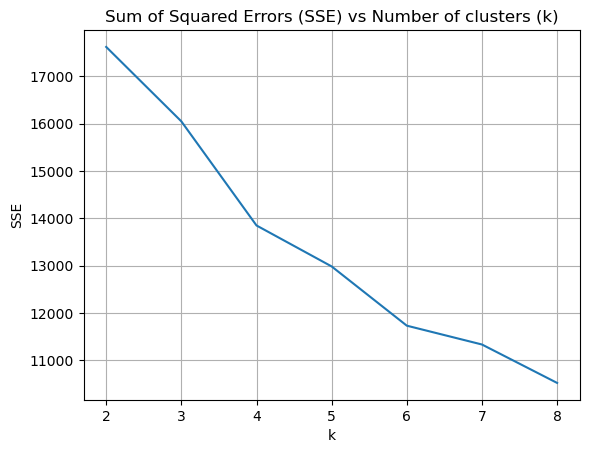
\includegraphics{sse_vs_k.png}
                        \captionof{figure}{SSE vs. Number of Clusters}
                    \end{center}

              \item Given the obtained results, the optimal number of clusters can be seen at the "elbow point", the point where before it the SSE decreases rapidly and after it decreases slowly. From the plot, we can see that this point is at $k=4$, meaning that there should be \textbf{4 underlying customer segments}.

                    To complement the reasoning, decreasing SSE means that data points are closer to the centroids and more data patterns are being captured. However, if too many clusters are used, the model may be at risk of overfitting, being perfect for the training data but bad at generalizing to new data.

              \item \textit{k-modes} is designed to work with categorical data, while \textit{k-means} is designed to work with numerical data. Since our dataset is mainly comprised of categorical data, \textbf{\textit{k-modes} would be a better approach}:

                    \begin{center}
                        \begin{minipage}{0.5\textwidth}
                            \texttt{Data columns \{total 16 columns\}:\\
                                \#   Column     Non-Null Count  Dtype \\
                                ---  ------     --------------  ----- \\
                                0   age        10316 non-null  int64 \\
                                1   job        10316 non-null  object \\
                                2   marital    10316 non-null  object \\
                                3   education  10316 non-null  object \\
                                4   default    10316 non-null  object \\
                                5   balance    10316 non-null  int64 \\
                                6   housing    10316 non-null  object \\
                                7   loan       10316 non-null  object \\
                                8   contact    10316 non-null  object \\
                                9   day        10316 non-null  int64 \\
                                10  month      10316 non-null  object \\
                                11  duration   10316 non-null  int64 \\
                                12  campaign   10316 non-null  int64 \\
                                13  pdays      10316 non-null  int64 \\
                                14  previous   10316 non-null  int64 \\
                                15  poutcome   10316 non-null  object\\}
                        \end{minipage}
                    \end{center}

                    \textit{k-means} uses Euclidean distances to cluster continuous data. Meaning that, the smaller the distance between two points, the more similar they are, and with high chances of landing in the same cluster.

                    Whereas \textit{k-modes} uses the Hamming distance, the number of dissimilarities between data points (the number of positions for an equal feature that are different, that lead to mis-matches). This is more suitable for categorical data, since it doesn't assume a linear relationship between the data points, as \textit{k-means} does.

          \end{enumerate}
    \item The 3 next exercises work upon the dataset data normalized according to \textbf{StandardScaler}
          \begin{enumerate}[leftmargin=0pt, label=\textbf{\alph*.)}]
              \item After performing the \textbf{PCA} on the data, the top 2 components correspond to the features 'age' and 'balance' with the variance ratios of 0.11679024 (aprox. 11,68\%) and 0.11075988 (aprox. 11,08\%), respectively.

                    This means that the top 2 components explain 22,76\% of the variance in the data.

              \item After performing \textit{k-means}, considering $k=3$, and plotting the results according to the first 2 principal components, the following plot was obtained:

                    \begin{center}
                        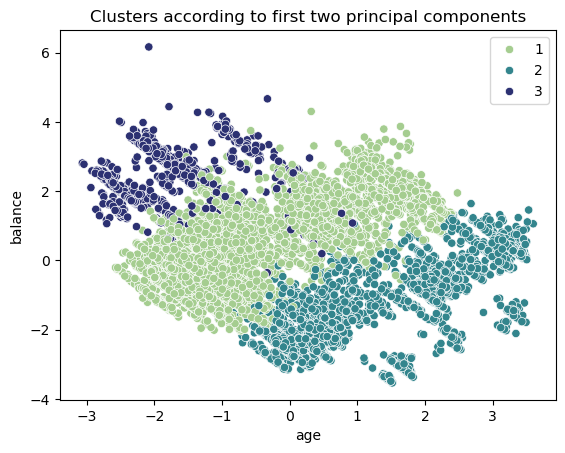
\includegraphics{clusters_first_two_components.png}
                        \captionof{figure}{Clusters according to the first 2 principal components}
                    \end{center}

                    We can conclude, by observing the plot, these 2 components aren't enough to clearly separate the clusters, as they overlap in some regions. This can be explained by the fact that, together, these components only explain 22.76\% of the variance in the data.

              \item When looking at the cluster conditional features for the original features 'job' and 'education', we get the following results:

                    \begin{center}
                        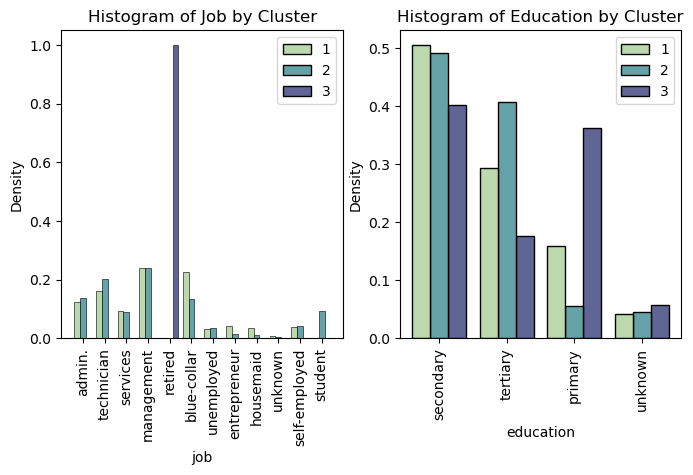
\includegraphics{cluster_conditional_features_job_education.png}
                        \captionof{figure}{Cluster conditional features for 'job' and 'education'}
                    \end{center}

                    Looking at the "job" histogram first, we can see some patterns starting to appear. For example, cluster 3 covers only retired people, while the other two clusters, 1 and 2, have a more diverse distribution of jobs, with some highlights being students belonging to cluster 1 and house-maids mostly belonging to cluster 2, with both clusters, overall, having no discernible pattern.

                    When taking the "education" histogram into account, the only major highlight is that most primary-educated people belong to cluster 3. The other education levels don't have a clear pattern, being spread across all clusters.

                    These results show that the clusters are not well separated when only considering the top 2 principal components. Some different ways to improve separation could be to increase the number of principal components used to cluster the data, to consider more clusters (being carefull not to overfit the data), or, the most effective way, to use a different clustering algorithm, better suited for the dataset, such as \textit{k-modes}.
          \end{enumerate}
\end{enumerate}
\newpage
\appendix
\section{Numpy Code for Exercise 1 - Pen and Paper}
\begin{lstlisting}[language=Python, caption=Python code for Exercise 1]
import numpy as np

# Initializing the observations, means, covariances, and mixture probabilities
observations = np.array([[1, 0], [0, 2], [3, -1]])
means = [np.array([2, -1]), np.array([1, 1])]
covariances = [np.array([[4, 1], [1, 4]]), np.array([[2, 0], [0, 2]])]
pis = [0.5, 0.5]

def multivariate_gaussian(x, mean, cov):
    d = len(mean)
    cov_det = np.linalg.det(cov)
    cov_inv = np.linalg.inv(cov)
    factor = 1 / ((2 * np.pi) ** (d / 2) * cov_det ** 0.5)
    exponent = -0.5 * (x - mean).T @ cov_inv @ (x - mean)
    return factor * np.exp(exponent)

def e_step(observations, means, covariances, pis):
    gammas = np.zeros((len(observations), len(means)))
    
    print("E-step:")
    
    # Step a
    p_x_given_c = []
    for i, x_i in enumerate(observations):
        p_x_k = []
        for k in range(len(means)):
            prob = multivariate_gaussian(x_i, means[k], covariances[k])
            p_x_k.append(prob)
            print(f"p(x{i + 1}|c{k + 1}) = {prob.round(3)}")
        p_x_given_c.append(p_x_k)
    
    # Step b
    p_c_and_x = []
    for i, x_i in enumerate(observations):
        p_c_x_k = []
        for k in range(len(means)):
            p_c_x = p_x_given_c[i][k] * pis[k]
            p_c_x_k.append(p_c_x)
            print(f"p(x{i + 1}, c{k + 1}) = {p_c_x.round(3)}")
        p_c_and_x.append(p_c_x_k)

    # Step c
    p_x = [sum(p_c_and_x[i]) for i in range(len(observations))]
    for i in range(len(observations)):
        for k in range(len(means)):
            gammas[i, k] = p_c_and_x[i][k] / p_x[i]
            print(f"\\gamma(c{k + 1}{i + 1}) = p(c{k + 1}|x{i + 1}) = 
            {gammas[i, k].round(3)}")
    
    return gammas

def m_step(observations, gammas):
    n_clusters = gammas.shape[1]
    N_k = gammas.sum(axis=0)
    new_means = []
    new_covariances = []
    new_pis = []

    print("\nM-Step:")
    
    for k in range(n_clusters):
        # Update mean
        weighted_sum = sum(gammas[i, k] * observations[i] 
            for i in range(len(observations)))
        new_mean = weighted_sum / N_k[k]
        new_means.append(new_mean.round(3))
        print(f"\\mu{k + 1} = {new_mean.round(3)}")

        # Update covariance
        weighted_cov_sum = sum(gammas[i, k] * np.outer(observations[i] 
            - new_mean, observations[i] - new_mean) for i in 
            range(len(observations)))
        new_covariance = weighted_cov_sum / N_k[k]
        new_covariances.append(new_covariance.round(3))
        print(f"Sigma{k + 1} = {new_covariance.round(3)}")

        # Update pi
        new_pi = (N_k[k] / len(observations)).round(3)
        new_pis.append(new_pi)
        print(f"\\pi{k + 1} = {new_pi:.3f}")

    return new_means, new_covariances, new_pis

# Run EM steps
for iteration in range(2):  # specify number of iterations
    print(f"\nIteration {iteration + 1}:")
    gammas = e_step(observations, means, covariances, pis)
    means, covariances, pis = m_step(observations, gammas)
    print("Updated Means:", means)
    print("Updated Covariances:", covariances)
    print("Updated Pis:", pis)
\end{lstlisting}
\newpage
\section{Numpy Code for Exercise 2a - Pen and Paper}
\begin{lstlisting}[language=Python, caption=Python code for Exercise 2a]
import numpy as np

# Updated parameters from Iteration 2
mu_1 = np.array([2.464, -0.728])
mu_2 = np.array([0.469, 1.145])

sigma_1 = np.array([[0.793, -0.407], [-0.407, 0.215]])
sigma_2 = np.array([[0.414, -0.619], [-0.619, 1.062]])

pi_1 = 0.433
pi_2 = 0.567

# Observations
x1 = np.array([1, 0])
x2 = np.array([0, 2])
x3 = np.array([3, -1])
observations = [x1, x2, x3]

# Multivariate Gaussian function
def multivariate_gaussian(x, mean, cov):
    d = len(mean)
    cov_det = np.linalg.det(cov)
    cov_inv = np.linalg.inv(cov)
    term1 = 1 / ((2 * np.pi) ** (d / 2) * np.sqrt(cov_det))
    term2 = np.exp(-0.5 * (x - mean).T @ cov_inv @ (x - mean))
    return term1 * term2

# Step 2a: Calculate the posterior probabilities for 
#each observation and cluster
posteriors = []

for x in observations:
    p_x_given_c1 = multivariate_gaussian(x, mu_1, sigma_1)
    p_x_given_c2 = multivariate_gaussian(x, mu_2, sigma_2)
    p_c1_x = p_x_given_c1 * pi_1
    p_c2_x = p_x_given_c2 * pi_2
    p_x = p_c1_x + p_c2_x
    posterior_c1 = p_c1_x / p_x
    posterior_c2 = p_c2_x / p_x
    posteriors.append((posterior_c1, posterior_c2))

print("Posterior probabilities (question 2a):")
for i, (p_c1, p_c2) in enumerate(posteriors, 1):
    print(f"p(c1 | x{i}) = {p_c1.round(3)}, p(c2 | x{i}) = {p_c2.round(3)}")

# Hard assignments based on MAP
clusters = {1: [], 2: []}
for i, (p_c1, p_c2) in enumerate(posteriors, 1):
    if p_c1 > p_c2:
        clusters[1].append(observations[i - 1])
    else:
        clusters[2].append(observations[i - 1])

print("\nClusters after hard assignment (question 2a):")
for cluster, points in clusters.items():
    print(f"Cluster {cluster}: {points}")
\end{lstlisting}
\end{document}
